\chapter{Arquitectura}
\label{chap:architecture}


\section{Introducción}
\label{sec:introduction}

En este capítulo trataremos la fase de diseño de este proyecto, así como los detalles de implementación de la arquitectura del mismo. Primero, presentaremos una vista general del proyecto por medio de un diagrama. A continuación se detallará la arquitectura en el cliente, así como la del servidor y los servicios que la componen. Posteriormente, se detallarán los módulos que conforman la aplicación, así como las métricas que se han decidido calcular y sus motivos. Con ello tenemos la intención de facilitar al lector una vista general de la arquitectura del proyecto.

Se presenta a continuación una vista general de la arquitectura de ChatStats:

\begin{figure}[H]
	\centering
	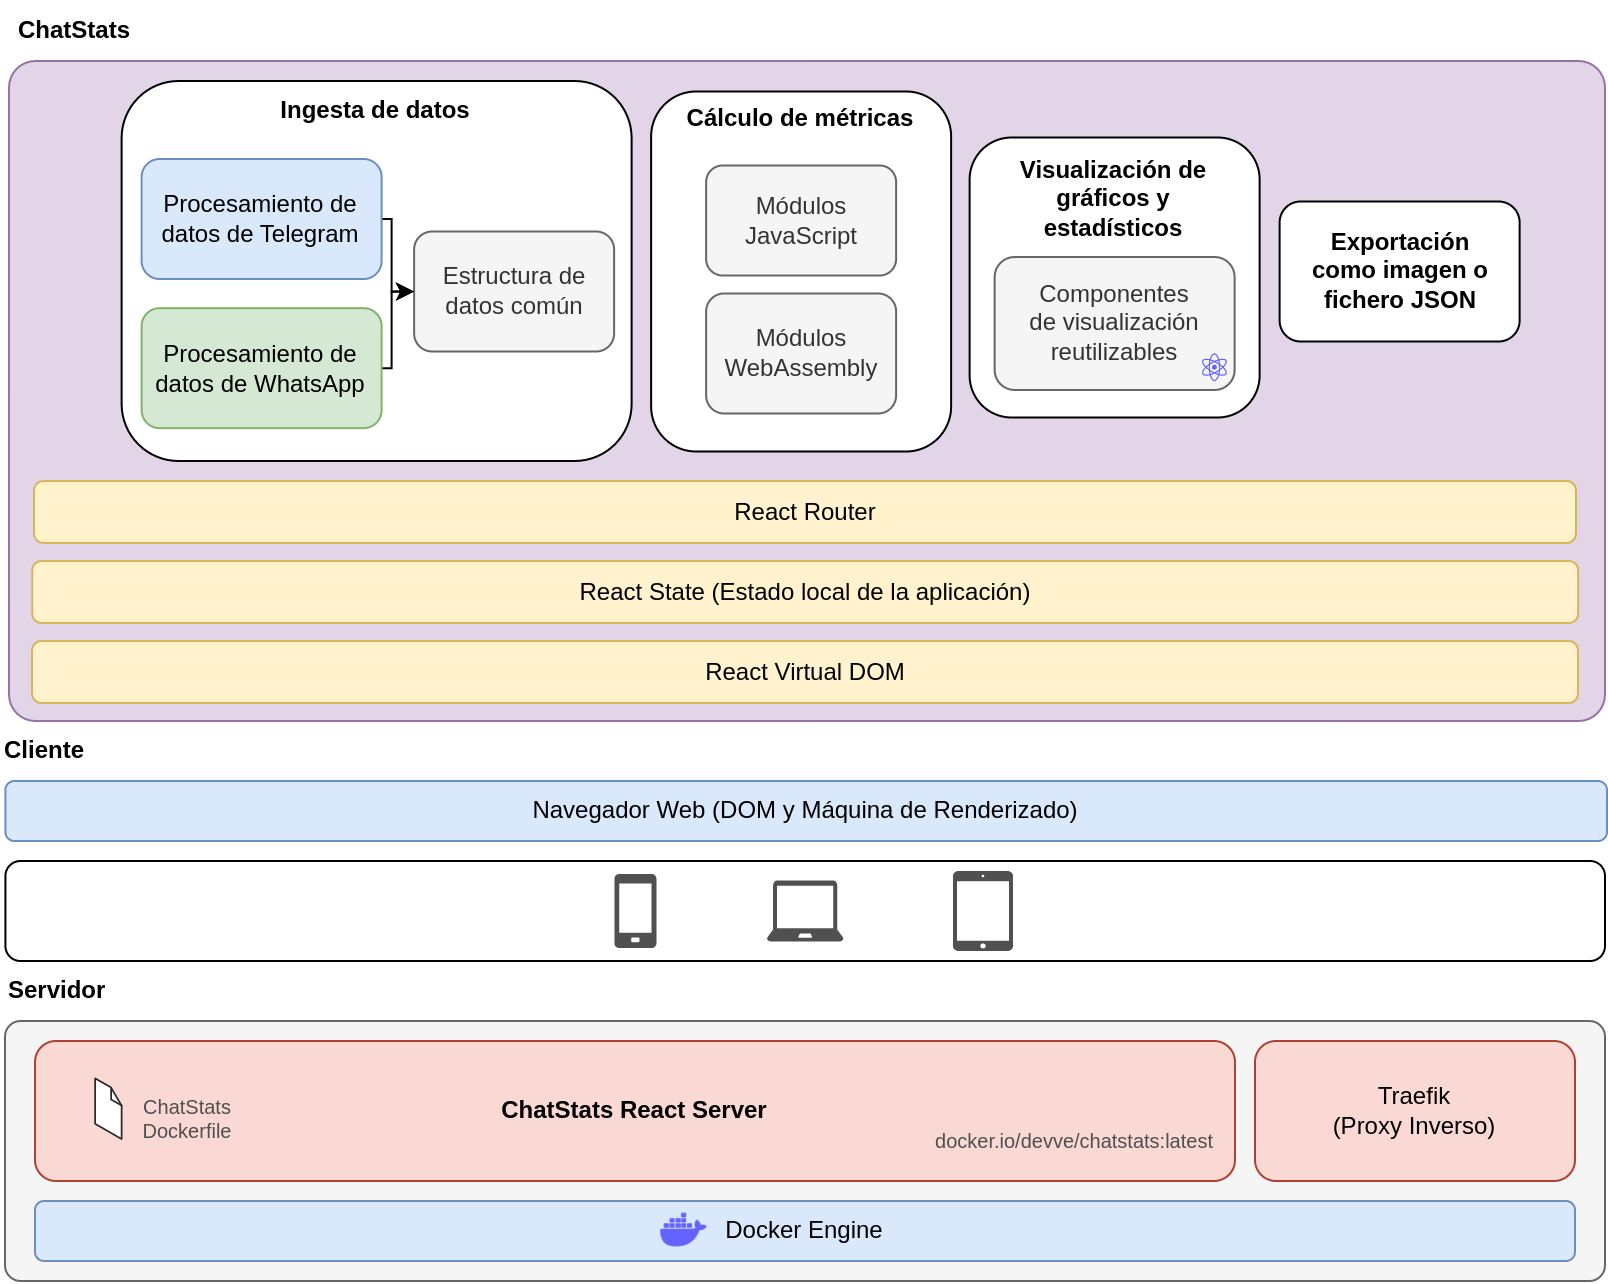
\includegraphics[width=\textwidth]{img/architecture.png}
	\caption{Arquitectura general}
	\label{fig:chap4:architecture_general}
\end{figure}


\begin{comment}
	Como se puede observar, el usuario debe exportar un chat desde la aplicación de WhatsApp (móvil) o Telegram para escritorio. Son estas las únicas versiones de las aplicaciones que permiten exportar las conversaciones. Con estos datos exportados, el usuario accede a ChatStats desde el navegador, ya sea en un dispositivo móvil o en un ordenador. El servidor le envía el cliente completo, por lo que no intercambia más peticiones en adelante. El usuario puede seleccionar e importar el archivo a la aplicación, que los estandariza, calcula métricas sobre la conversación y ofrece una visualización de los mismos. Finalmente, el usuario puede compartir las visualizaciones, así como exportar los datos calculados para su uso personal.
	
	
	Se desarrolla toda la aplicación en \textit{JavaScript}, puesto que puede ejecutarse en todos los navegadores salvo que lo tengan deshabilitado. Otros lenguajes como \textit{PHP} o Python requieren de un servidor para realizar operaciones y que estos envíen una plantilla rellena con los resultados.
\end{comment}


\section{Arquitectura en el cliente}

A continuación se presenta la arquitectura que podemos encontrar en un cliente cualquiera. Puede tomarse la \autoref{fig:chap4:architecture_client} para observar las capas que la componen.

\begin{figure}[h]
	\centering
	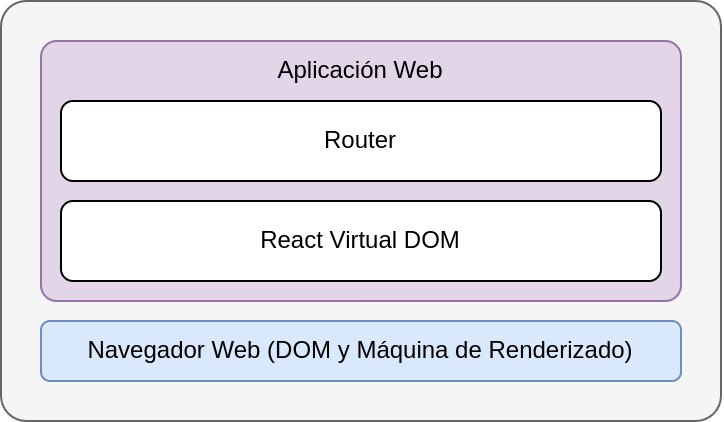
\includegraphics[width=0.6\textwidth]{img/client.png}
	\caption{Arquitectura en el cliente}
	\label{fig:chap4:architecture_client}
\end{figure}

\paragraph{Navegador.} El navegador juega un papel fundamental para el acceso y ejecución de cualquier aplicación web. Aunque no se entra en detalle en su estructura interna, sí que vamos a detallar la integración con \acrfull{pwa}. Esta integración que ofrecen algunos navegadores como los basados en Chromium, permite instalar aplicaciones web, con ventajas como:

\begin{itemize}
	\item La aplicación saldrá en el escritorio en teléfonos Android e iOS, así como en el cajón de aplicaciones del navegador.
	\item Posibilidad de acceso a notificaciones \textit{push} para el sistema (que no utilizaremos).
	\item Posibilidad de guardar en \textit{cache} el código del cliente, permitiendo su uso sin conexión a Internet.
\end{itemize}

Es por ello que ChatStats puede ser instalada en los dispositivos con un navegador con soporte \acrshort{pwa}, permitiendo su instalación y ejecución sin acceso a Internet. Para ello, ChatStats registra un \textit{service worker} o trabajador de servicio que guarda el código en el cliente, así como un archivo de manifiesto que recoge un título, descripción e iconos de la aplicación.

Hay que mencionar también que Mozilla no ofrece soporte para \acrshort{pwa} en su navegador Firefox\cite{firefoxNoPWA}, aunque este puede ser habilitado mediante una extensión\cite{firefoxPWAextension}.

\paragraph{Aplicación Web.} En esta última capa se encuentra nuestra aplicación, cuya arquitectura de procesamiento se explica en la \autoref{chap:architecture:processing}. Explicamos a continuación los componentes lógicos que se encuentran en el cliente:

\subparagraph{React State.} Se trata de la capa que maneja el estado de nuestra aplicación, en el que se almacenan los resultados de los cálculos, importación de archivos y otros, como se verá en la \autoref{chap:architecture:processing}. Permite además que nuestra aplicación reaccione a los cambios sucedidos en esta capa de estado, pudiendo refrescar componentes que hagan uso de la información almacenada si fuese necesario.

\subparagraph{Router.} ChatStats es una aplicación multipágina. Esto quiere decir que cuenta con diferentes rutas web en las que se muestran diferentes páginas. La página principal consolida la ruta `\textit{/}', mientras que `\textit{/graphs}' enruta la página para la visualización de los gráficos. Usamos el enrutador proporporcionado por React para permitir la navegación por la aplicación, mapeando las rutas a los componentes de React que se deben visualizar en cada una. Estos se explicarán en la \autoref{chap:architecture:processing}.

\subparagraph{React Virtual DOM.} El DOM virtual es un concepto de programación en el que una representación virtual de la interfaz de usuario (UI) es guardada en memoria y sincronizada con el DOM del navegador. Esto nos permite definir qué queremos en la interfaz de usuario y React conseguirá que el DOM virtual y el DOM del navegador se sincronicen.


Por último, cabe añadir que se han implementado reglas de estilo que tienen en cuenta el tamaño de la pantalla y se adaptan al mismo, permitiendo mantener la usabilidad del cliente en teléfonos, tabletas y ordenadores.





\section{Arquitectura en el servidor}
\label{chap:architecture:server}

Se muestra a continuación una grafo de la arquitectura en el servidor, donde se muestran las capas que lo componen.

\begin{figure}[H]
	\centering
	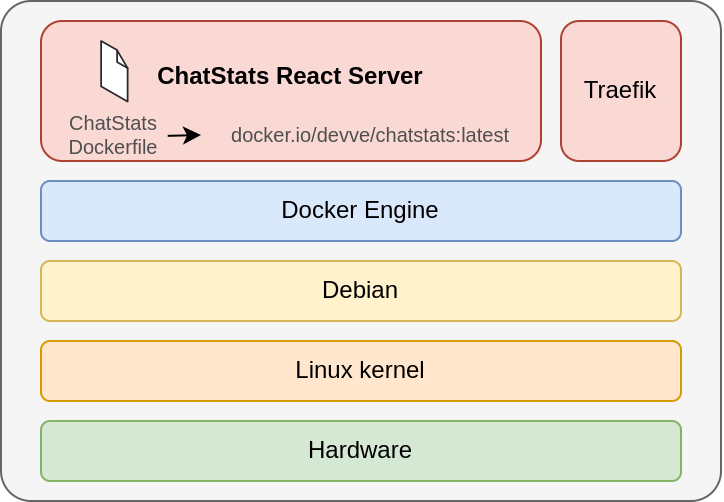
\includegraphics[width=0.6\textwidth]{img/server.png}
	\caption{Arquitectura en el servidor}
	\label{fig:chap4:architecture_server}
\end{figure}

Se ha decidido no instalar el software directamente sobre el sistema operativo, evitando problemas de dependencias y distintas versiones de las mismas para los componentes del sistema operativo. Asimismo, se evitan problemas de seguridad que puedan venir por vulnerabilidades en el código fuente y sus dependencias.

Hemos elegido virtualización ligera para ejecutar nuestro código en contenedores, por las razones que se exponen:

\begin{itemize}
	\item Se contienen las dependencias de terceros en una imagen.
	\item En caso de vulnerabilidad, solo se expone el contenedor y no el sistema completo.
	\item Los recursos se ocupan dinámicamente en función a las necesidades, al contrario que con la virtualización completa.
	\item Permite el despliegue en cualquier sistema operativo compatible con Linux, salvo arquitecturas ARM (que no es frecuente en servidores).
\end{itemize}

\paragraph{ChatStats React Server.} Se trata del servidor de React que sirve el contenido. Tras construir una imagen con la versión de producción a partir del código fuente, este contenedor sirve el contenido estático final, que enviará al cliente completamente cuando este solicite la aplicación web. Se ha implementado por medio de un fichero Dockerfile, que parte de una imagen de \textit{NodeJS}, instala las dependencias y sirve el contenido. Con esta secuencia de instrucciones, se ha creado una imagen para uso en contenedores Docker, que puede encontrarse públicamente en el repositorio de imágenes DockerHub.

\paragraph{Traefik} Se ha decidido usar Traefik como \textit{proxy} inverso, que se sitúa frente al servidor de ChatStats para redirigir las peticiones realizadas a su contenedor correspondiente en el puerto adecuado.

Además, Traefik gestiona los certificados \acrshort{ssl} haciendo uso de \textit{Let's Encrypt}: autoridad sin ánimo de lucro que provee certificados para la capa \acrshort{tls} sin coste alguno.








\section{Arquitectura de la aplicación}
\label{chap:architecture:processing}


Con el objetivo de mantener la privacidad de los datos del usuario, se ha planteado una arquitectura centrada en el cliente, donde el servidor únicamente envía la totalidad de la aplicación al cliente en la primera petición. Esto supone un mayor coste computacional en el cliente para realizar todas las operaciones necesarias, por lo que la eficiencia del código es necesaria. Además, esta arquitectura se puede extender, en un futuro, ofreciendo analíticas adicionales si el usuario opta por enviar información al servidor para su procesamiento. Este caso de extensión se detallará más adelante.

A continuación se muestra la arquitectura de la lógica de negocio en la aplicación:

\begin{figure}[H]
	\centering
	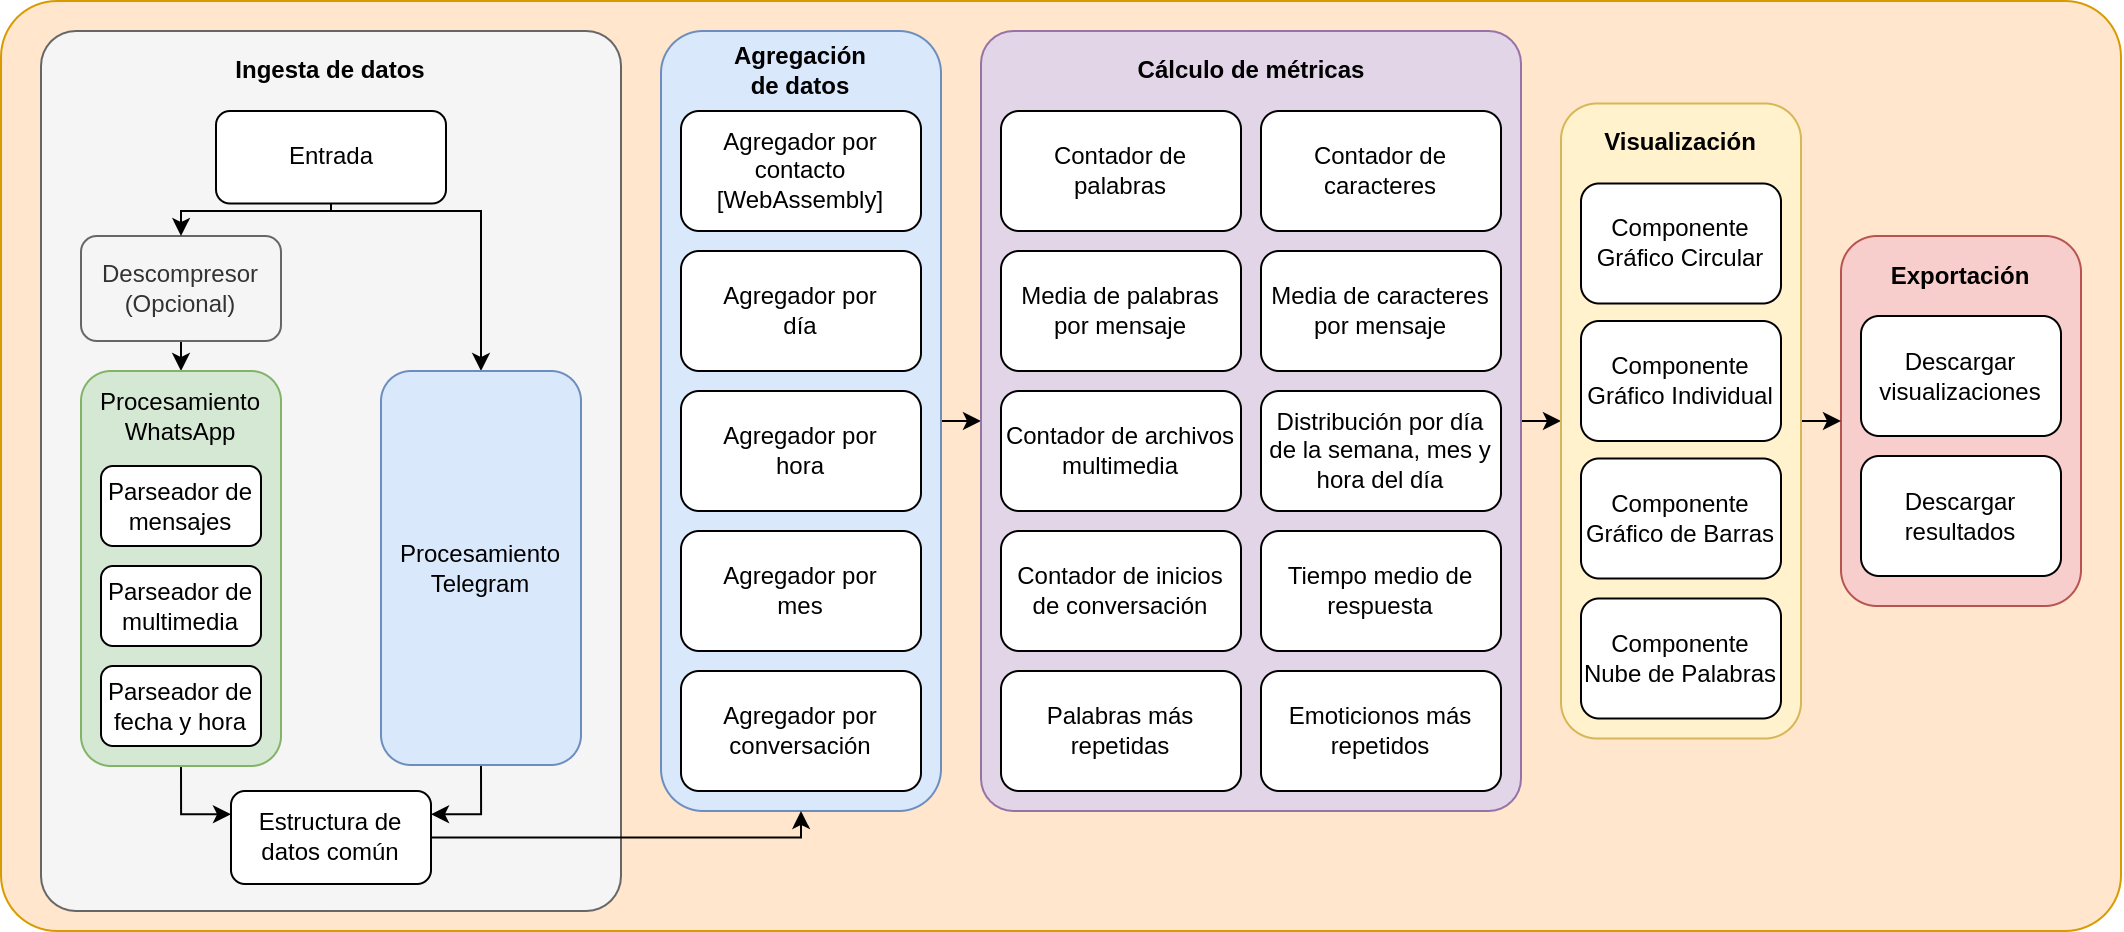
\includegraphics[width=\textwidth]{img/architecture_processing.png}
	\caption{Arquitectura de la aplicación}
	\label{fig:chap4:architecture_processing}
\end{figure}

\subsection{Ingesta de datos}
\label{chap:architecture_ingesta}

El módulo importador se encarga de leer el fichero de entrada exportado desde la aplicación WhatsApp o Telegram y convertirlos a una estructura de datos normalizada para el procesamiento de los módulos posteriores. Dicho fichero puede estar en tres formatos diferentes:

\begin{itemize}
	\item \textit{txt} si se trata de un chat exportado de WhatsApp en un dispositivo Android.
	\item \textit{zip} si se trata de un chat exportado de WhatsApp desde un dispositivo iOS.
	\item \textit{\acrshort{json}} si se trata de un chat exportado de Telegram desde la aplicación para escritorio.
\end{itemize}

Aunque Telegram también soporta la exportación de conversaciones en \textit{HTML}, ChatStats no soporta este formato, puesto que está diseñado para la visualización y no para el tratamiento y procesado del mismo.


Mientras que Telegram ofrece los datos de exportación en formato \acrshort{json}, facilitando así la operabilidad de los mismos; WhatsApp no ofrece una estructura de datos ni consistencia entre distintas versiones de su aplicación. Es por ello que, en busca de la reutilización del código y escalabilidad del mismo, este módulo tiene como salida la siguiente estructura de datos:

\begin{lstlisting}[language=JavaScript]
	{
		date: new Date("2022-10-17T10:37:00"),
		from: "Juan Pedro",
		text: "IMG-20221020-WA0013.jpg",
		type: "message",
		media_type: "image"
	}
\end{lstlisting}

Esta estructura de datos conforma el máximo común divisor de la información que podemos obtener de Telegram y WhatsApp, por lo que es un buen punto de partida.

Además, en una primera instancia, cabe destacar que ChatStats únicamente hace uso de los metadatos del contenido multimedia, tales como formato de archivo, extensión y fecha. Estos datos se incluyen en el fichero que la aplicación espera a la entrada. Esto se detallará más adelante en este mismo módulo.


\paragraph{Entrada}\mbox{}\\

Este submódulo se encarga de cargar el fichero seleccionado por el usuario, que el navegador ofrece desde una ruta virtual y protegida, para que la aplicación no pueda acceder a todos los archivos del dispositivo. En caso de tratarse de un fichero de texto plano, este módulo abre el archivo como una cadena de caracteres. En caso de tratarse de un fichero comprimido, se lo envía al módulo ``Descompresor'' esperando un archivo de texto plano como salida. Por último, en caso de tratarse de cualquier otro tipo de fichero, el módulo alerta al usuario de que el archivo de entrada no es válido.

Este submódulo hace uso de una instancia de \textit{FileReader}; clase que ofrecen los navegadores, permitiendo abrir el fichero como secuencia de caracteres.

\paragraph{Descompresor (Opcional)}\mbox{}\\

Este submódulo se encarga de la descompresión de ficheros \textit{zip}, que descomprime bajo petición del módulo anterior. Finalmente, el módulo devuelve un fichero llamado \textit{\_chat.txt}, que, como se ha comentado anteriormente, contiene toda la información necesaria para el análisis (con o sin multimedia).

El descompresor hace uso de la librería \textit{jszip} para la descompresión del fichero. La lógica añadida a esta aplicación nos permite encontrar el fichero de texto plano dentro del fichero comprimido y devolver el mismo al módulo de ``Procesamiento WhatsApp''.


\paragraph{Procesamiento Telegram}\mbox{}\\

El objetivo de este submódulo es transformar el modelo de datos que exporta Telegram a el modelo de datos que utiliza ChatStats para el resto de sus módulos. Un ejemplo del objeto \acrshort{json} exportado por Telegram puede observarse en el \autoref{chap:telegram_json}.

En este caso, el submódulo de ``Entrada'' nos envía una cadena de caracteres en formato \acrshort{json}. Haciendo uso de la librería \textit{JSON} nativa para \textit{JavaScript}, podemos parsear el contenido de la cadena para obtener el objeto \acrshort{json}.

Debido a que Telegram ofrece una estructura que puede utilizarse para chats individuales o grupales, además de ofrecer soporte para mensajes multimedia, ChatStats hereda ciertas claves de dicha estructura. Es por ello que este submódulo elimina todas las claves no necesarias del objeto mensaje original de Telegram, quedándonos únicamente con las siguientes claves:

\begin{itemize}
	\item \textbf{``from'':} almacena el nombre del contacto. Admite cualquier secuencia de caracteres.
	\item \textbf{``type'':} almacena el tipo de mensaje. Actualmente su valor es \textit{``message''}, pero se ha considerado útil para futura escalabilidad del proyecto, dando soporte a videollamadas y cambio de nombre de grupo (anuncios), entre otros.
	\item \textbf{``date'':} almacena la fecha y hora del mensaje.
	\item \textbf{``media\_type'':} almacena el tipo de contenido multimedia. Puede tomar como valor: \textit{``voice\_message''}, \textit{``video\_file''}, \textit{``sticker''} o \textit{``image''}
\end{itemize}

\paragraph{Procesamiento WhatsApp}\mbox{}\\

Este submódulo se encarga, al igual que el submódulo anterior, de obtener mensajes con la estructura descrita al principio del módulo, a partir del archivo exportado de WhatsApp.

A continuación se muestra un mensaje exportado desde WhatsApp por un dispositivo Android:

\begin{lstlisting}
	17/07/2022, 01:28 - Alice: Este es un mensaje de prueba.
\end{lstlisting}

Así como un mensaje exportado desde WhatsApp por un dispositivo iOS:

\begin{lstlisting}
	[29/12/22, 0:14:55] Bob: Te escribo desde mi iPhone.
\end{lstlisting}

Podemos observar que, en el caso de WhatsApp, ambos mensajes se componen de la fecha, la hora, el nombre del contacto y el propio cuerpo del mensaje, aunque con distinto formato.

\subparagraph{Parseador de mensajes} Se implementa, como puede verse en el \autoref{chap:regex} un parseador mediante una expresión regular. Dicho parseador encuentra los mensajes en el texto recibido del submódulo de ``Entrada'' y los divide en: fecha y hora, contacto y cuerpo del mensaje. Podemos observar que no encontramos ninguna referencia al contenido multimedia aún, puesto que para ello hay que parsear el cuerpo del mensaje en busca de metadatos. Además, la fecha y la hora son una cadena de caracteres, que transformaremos a continuación.

\subparagraph{Parseador de fecha y hora} Este componente tiene como entrada la fecha y la hora del mensaje obtenido en el paso anterior. Devuelve un objeto de tipo \textit{Date}, nativo de JavaScript. Esto nos permite realizar operaciones de tiempo con facilidad en otros módulos.

Este submódulo utiliza la librería \textit{momentjs} para parsear los posibles distintos formatos de fecha que utilizan Telegram y WhatsApp en sus cadenas de caracteres. Además, considera el \textit{locale} del cliente, invirtiendo mes y día para el caso \textit{en\_US}.

\subparagraph{Parseador de archivos multimedia} El objetivo de este componente es escribir el tipo de contenido en la clave \textit{``media\_type''} del objeto mensaje expuesto anteriormente, buscando la extensión del archivo adjunto.

Se indican a continuación mensajes de ejemplo para cada tipo de archivo adjunto, únicamente para Android:

\begin{lstlisting}
	17/10/2022, 21:11 - Juan Pedro: PTT-20221017-WA0078.opus (file attached)
	20/10/2022, 10:37 - Juan Pedro: IMG-20221020-WA0013.jpg (file attached)
	14/11/2022, 18:58 - Juan Pedro: VID-20221114-WA0039.mp4 (file attached)
	24/11/2022, 19:13 - Jaime Conde: STK-20220717-WA0090.webp (file attached)
\end{lstlisting}

En el fichero de texto plano con contenido multimedia, observaremos que el cuerpo incluye el nombre del fichero que se ha exportado con la extensión del formato del mismo. Por ello, categorizamos como \textit{voice\_message}, \textit{video\_file}, \textit{sticker} o \textit{image} en función a la extensión; \textit{.opus}, \textit{.mp4}, \textit{.webp} o \textit{.jpg}, respectivamente. Usamos estos valores puesto que son los que Telegram utiliza para su formato de mensajes.

Si el fichero no incluye estos metadatos, cada vez que un mensaje sea contenido multimedia, aparecerá \textit{\textless Media omitted \textgreater} (multimedia omitido). Estos pueden ser fotos, vídeos, música, notas de voz o documentos. Se definirán como \textit{undefined} o indefinidos, ignorándose en las visualizaciones y módulos posteriores. Se muestra un ejemplo a continuación:

\begin{lstlisting}
	17/07/2022, 01:33 - Juan Pedro: <Media omitted>
\end{lstlisting}

\subsection{Agregación de datos}

Los mensajes se encuentran segregados en una lista, por lo que a continuación, el módulo de agregador se encargará de agregar los mensajes en diferentes grupos. En el código los hemos llamado polarizadores. Se describen los distintos submódulos a continuación:

\paragraph{Agregador por contacto}\mbox{}\\

\textit{ChatStats} se encarga de calcular las estadísticas de cada contacto para visualizarlas y mostrarlas en comparación con el resto de contactos. Hablamos de numerosos contactos, puesto que es compatible con chats individuales y grupales.

El resultado de este submódulo será un objeto \acrshort{json} con una clave por cada contacto (su nombre), que contendrá un array de los mensajes enviados por este. Se indica un ejemplo:

\begin{lstlisting}[language=JavaScript]
	{
		"Jaime": [...messagesByJaime],
		"Juan Pedro": [...messagesByJuanPedro],
		...
	}
\end{lstlisting}

donde los array de mensajes contienen objetos con la estructura de datos común mencionada en el módulo anterior,  \autoref{chap:architecture_ingesta}.

Cabe anotar que este submódulo está desarrollado en Rust, haciendo uso de la tecnología \acrfull{wasm}; puesto tras medir los tiempos de ejecución de las distintas funciones, se ha comprobado que este era el mayor. Además, sirve como parámetro de entrada para la mayoría de los agregadores que explicaremos a continuación. Se utiliza la librería \textit{``wasm-pack''} de Rust, que genera automáticamente el paquete JavaScript del que hará uso nuestra aplicación en React. Este paquete, una vez construido, exporta las funciones públicas que estén decoradas para su uso en \acrshort{wasm}. Estas funciones enlazan a un binario que \textit{``wasm-pack''} construye también por nosotros.

\paragraph{Agregador por día}\mbox{}\\

Este agregador toma como entrada la salida del submódulo anterior: los mensajes agregados por contacto. Con ello se procede a agregarlos, además, por día de la semana: de lunes a domingo. Se usará el nombre del día de la semana como clave anidada.

El resultado son objetos con la siguiente estructura:

\begin{lstlisting}[language=JavaScript]
	{
		"Jaime": {
			"monday": [...messagesByJaimeOnMonday],
			"tuesday": [...messagesByJaimeOnTuesday],
			...,
			"sunday": [...messagesByJaimeOnSunday]
			},
		"Juan Pedro": {
			"monday": [...messagesByJuanPedroOnMonday],
			"tuesday": [...messagesByJuanPedroOnTuesday],
			...,
			"sunday": [...messagesByJuanPedroOnSunday]
		},
		...
	}
\end{lstlisting}

El objetivo de esta estructura de datos es visualizar la distribución de los mensajes a lo largo de la semana, en media.

\begin{comment}
	Se deja para futuras líneas un gráfico en el que se pueda elegir el año a analizar, o un scroll vertical por años.
\end{comment}

\paragraph{Agregador por hora}\mbox{}\\

Este agregador toma también como entrada los mensajes agregados por contacto. Con ello se procede a agregarlos, además, por hora del día, usando la hora en formato 24 horas como clave anidada de agregación: de 00 a 23 horas.

El resultado son objetos con la siguiente estructura:

\begin{lstlisting}[language=JavaScript]
	{
		"Jaime": {
			"00": [...messagesByJaimeAt00],
			"01": [...messagesByJaimeAt01],
			...,
			"23": [...messagesByJaimeAt23]
		},
		"Juan Pedro": {
			"00": [...messagesByJuanPedroAt00],
			"01": [...messagesByJuanPedroAt01],
			...,
			"23": [...messagesByJuanPedroAt23]
		},
		...
	}
\end{lstlisting}

El objetivo de esta estructura de datos es visualizar la distribución de los mensajes a lo largo del día, en media.

\paragraph{Agregador por mes}\mbox{}\\

Este agregador toma también como entrada los mensajes agregados por contacto. Con ello se procede a agregarlos, además, por MM/YYYY, por lo que deja de tratarse de un agregador acotado: pueden haber tantas claves anidadas como meses se haya hablado.

El resultado son objetos con la siguiente estructura:

\begin{lstlisting}[language=JavaScript]
	{
		"Jaime": {
			"10/2022": [...messagesByJaimeOnOctober2022],
			"11/2022": [...messagesByJaimeOnNovember2022],
			...
		},
		"Juan Pedro": {
			"10/2022": [...messagesByJuanPedroOnOctober2022],
			"11/2022": [...messagesByJuanPedroOnNovember2022],
			...
		},
		...
	}
\end{lstlisting}

El objetivo de esta estructura de datos es visualizar la distribución de los mensajes a lo largo del tiempo, con una agregación mensual.

\paragraph{Agregador por conversación}\mbox{}\\

Este submódulo analiza las diferencias de tiempos entre los mensajes, categorizándolos como inicio de conversación si son el primer mensaje en las últimas 5 horas, o como respuesta si se trata de un intervalo de tiempo menor. Esto nos permitirá calcular cuántas conversaciones ha iniciado cada contacto, así como el tiempo de respuesta medio de cada uno; módulos que se verán más adelante.

Aunque un sesgo temporal no es una solución perfecta, acierta gran parte de las veces sin necesitar gran capacidad de cómputo.

\subsection{Cálculo de métricas}
\label{chap:architecture_metrics}

Este módulo prepara analiza y extrae los datos para ser representados por los componentes del módulo de visualización, que sigue a este. No se realizarán mayores detalles en la implementación, puesto que se han utilizado funciones nativas de JavaScript para su implementación, que puede verse en el código del \autoref{chap:code}. 

Cabe destacar que, una vez calculadas las métricas, estas pasan al estado local de la aplicación, permitiendo desencadenar acciones en la interfaz de usuario, tales como la representación visual de las métricas por medio del módulo que sigue a este.

Se describen a continuación las métricas elegidas, así como el razonamiento de su elección:

\paragraph{Contador de mensajes}

Este submódulo cuenta el número de mensajes enviado por cada contacto. Se ha optado por calcular esta métrica puesto que puede ayudar a observar diferencias drásticas en la cantidad de mensajes que aporta cada contacto.

\paragraph{Contador de palabras}

Este submódulo cuenta las palabras que hay en los mensajes de cada contacto y calcula la suma total de las mismas, obteniendo el número de palabras totales enviadas por cada contacto.

\paragraph{Contador de caracteres}

Este submódulo cuenta los caracteres que hay en los mensajes de cada contacto y calcula la suma total de los mismos, obteniendo el número de caracteres totales enviados por cada contacto. Aunque suele indicar resultados similares al módulo anterior, en algunas ocasiones es distinto, por lo que se ha decidido incluir también.

\paragraph{Media de palabras por mensaje}

Este submódulo calcula y muestra el número medio de palabras por mensaje para cada contacto. Esta métrica puede ayudar, junto con el número de mensajes totales, a saber si un contacto tiende a mandar más mensajes con menor número de palabras, o menos mensajes con más palabras.


\paragraph{Media de caracteres por mensaje}

Este submódulo calcula y muestra el número medio de caracteres por mensaje para cada contacto. Aunque suele indicar resultados similares al módulo anterior, en algunas ocasiones puede resaltar personas que tienden a usar palabras más largas.


\paragraph{Número de conversaciones iniciadas}

Este submódulo calcula el número de veces que cada contacto ha iniciado la conversación, con los criterios y datos obtenidos del módulo ``Agregador por conversación''. Se ha decidido calcular esta métrica puesto que es una buena forma de medir la iniciativa de una persona, así como su interés en el grupo o persona individual.


\paragraph{Velocidad media de respuesta}

Este submódulo calcula la velocidad media de respuesta de cada contacto, con los criterios y datos obtenidos del submódulo ``Agregador por conversación''. Se ha decidido calcular esta métrica puesto que es una buena forma de medir la atención a la aplicación de mensajería instantánea, así como la importancia que le da al grupo.

Se eliminan todos los  mensajes desde que un usuario comienza a responder hasta que termina, para no tenerlos en cuenta en el cálculo del tiempo de respuesta (puesto que se responde a sí mismo a partir del primer mensaje).


\paragraph{Contador de multimedia}

En caso de que existan objetos \acrshort{json} con el campo ``\textit{media\_type}'' distinto de \textit{undefined}, este submódulo cuenta cuántos archivos multimedia de cada tipo ha mandado cada contacto.

\paragraph{Generador de estructuras de datos por día, hora y mes}

Se elige calcular y mostrar distribuciones en los meses puesto que ayudan a observar la evolución en el tiempo de la cantidad de mensajes intercambiados, así como la distribución en los días de la semana ayuda a ver los días más activos en un periodo de una semana. Por último, la distribución en las 24 horas del día ayuda a analizar las horas pico de conversación, así como las horas de inicio y final del día para cada contacto.

\paragraph{Contador de palabras más repetidas}

Este submódulo procesa todas las palabras de los mensajes, elimina las palabras más comunes del español y el inglés, así como otros mensajes que WhatsApp añade, como \textit{Media ommited} o \textit{This message has been deleted}.

Las listas de palabras más comunes del español e inglés se han recopilado de distintas fuentes, combinado y eliminado repeticiones.

Esta información resulta útil para resaltar los temas principales tratados en el chat.

\paragraph{Contador de emoticonos más usados}

Este módulo aplica una expresión regular unicode a todos los mensajes, seleccionando los emoticonos y contando el número de veces que aparecen.

Se elige calcular y mostrar esta visualización puesto que los emoticonos constituyen en un chat la forma más similar a la expresión no verbal.

\subsection{Visualización}

El módulo visualizador está formado por un conjunto de componentes visuales reutilizables para distintos tipos de estadísticas, independientemente del formato de las mismas. Para ello, se desarrolla la siguiente estructura, común a todos los componentes:

\begin{figure}[H]
	\centering
	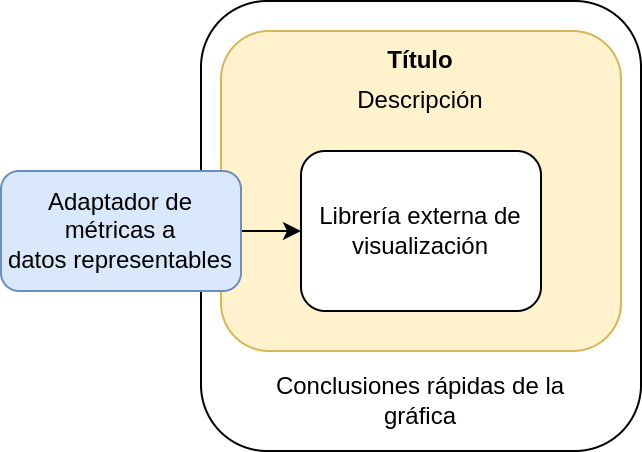
\includegraphics[width=0.5\textwidth]{img/visualizadores.png}
	\caption{Estructura de un componente de visualización}
	\label{fig:chap4:visualization}
\end{figure}

donde el adaptador de métricas a datos representables, asegura que tanto los gráficos circulares como los de barras e individuales, tengan consistencia en los colores utilizados. Además, este adaptador permite eliminar la lógica del cálculo de métricas y del componente de visualización, atomizando, en la medida de lo posible, el código y la arquitectura del proyecto. La estructura de datos que ofrece el módulo a la salida es la siguiente:

\begin{lstlisting}[language=JavaScript]
	{
		"labels": ["etiqueta 1", "etiqueta 2", ["valores anidados"]]{
		"datasets": ["valor 1", "valor 2", ["valores anidados"]],
		"backgroundColors": ["color 1", "color 2", ["valores anidados"]],
		"fillColors": ["color 1", "color 2", ["valores anidados"]]
	}
\end{lstlisting}

donde los valores anidados permiten introducir múltiples datos para una única etiqueta.

Los componentes esperan un título y una descripción, un set de datos como el mostrado anteriormente y el máximo y mínimo de los datos representados aportados. Con estos últimos datos, en caso de estar presentes, el componente muestra una frase de conclusión sobre el gráfico mostrado.

Con ello, se han desarrollado los siguientes componentes que se muestran en la \autoref{fig:chap4:visualization_examples}.


\begin{figure}[h]
	\centering
	\subfloat[\centering Gráfico circular]{{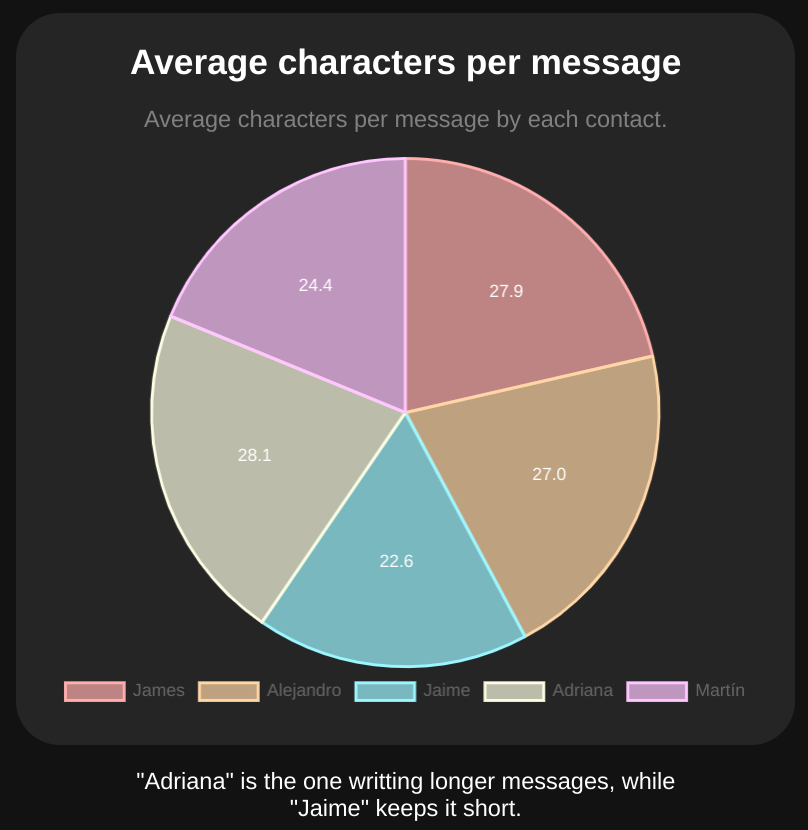
\includegraphics[width=6cm]{img/circular_graph.png} }}
	\qquad
	\subfloat[\centering Gráfico de barras vertical]{{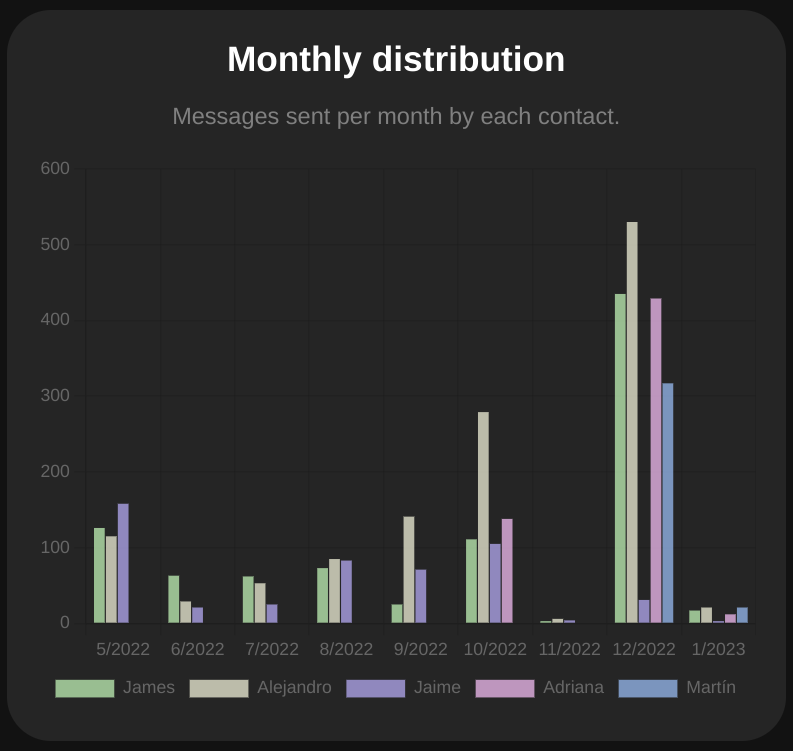
\includegraphics[width=6cm]{img/bar_graph_1.png} }}
	\qquad
	
	\subfloat[\centering Gráfico de barras horizontal]{{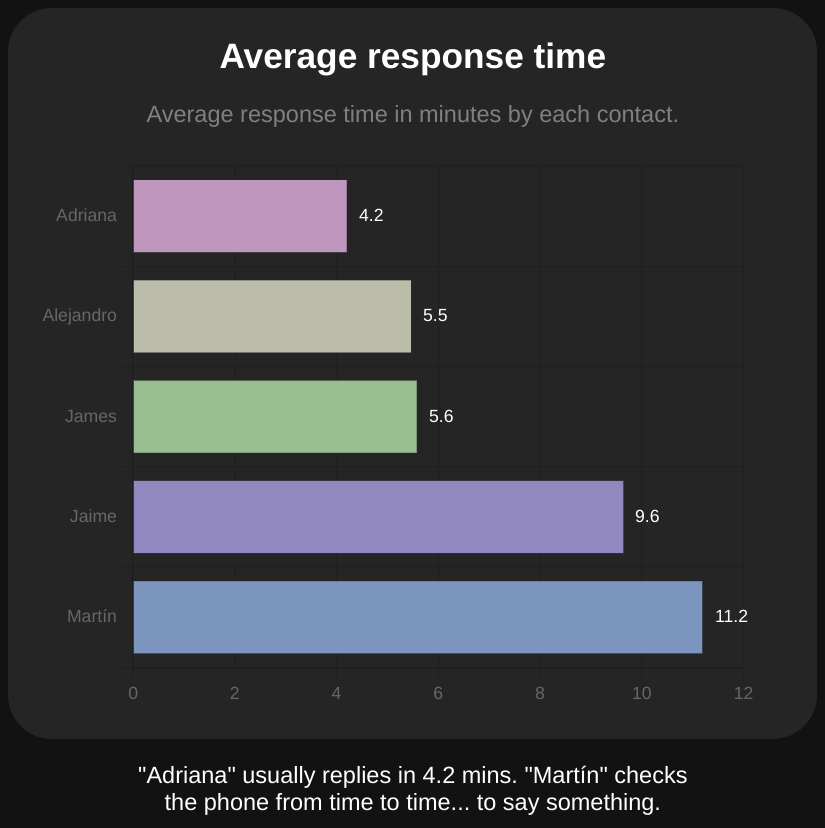
\includegraphics[width=6cm]{img/bar_graph_2.png} }}
	\qquad
	\subfloat[\centering Gráfico individual]{{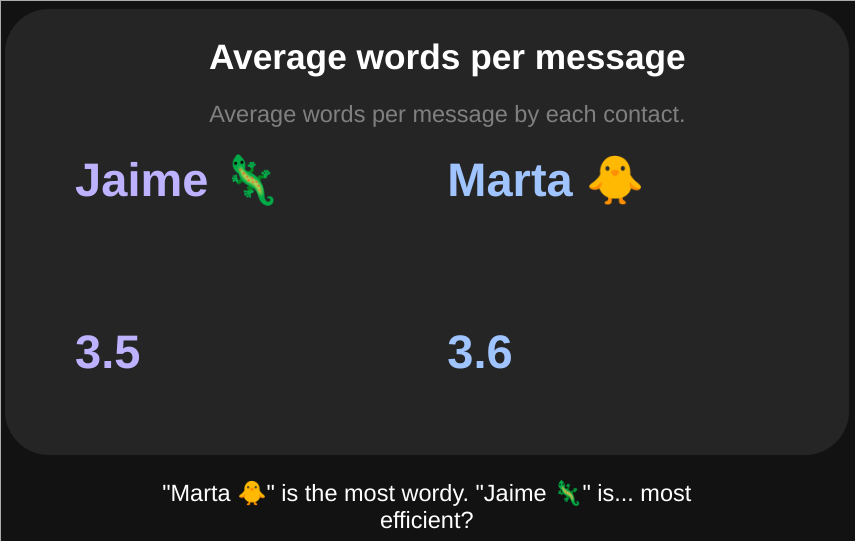
\includegraphics[width=6cm]{img/individual_graph.png} }}
	\qquad
	
	
	\subfloat[\centering Nube de palabras]{{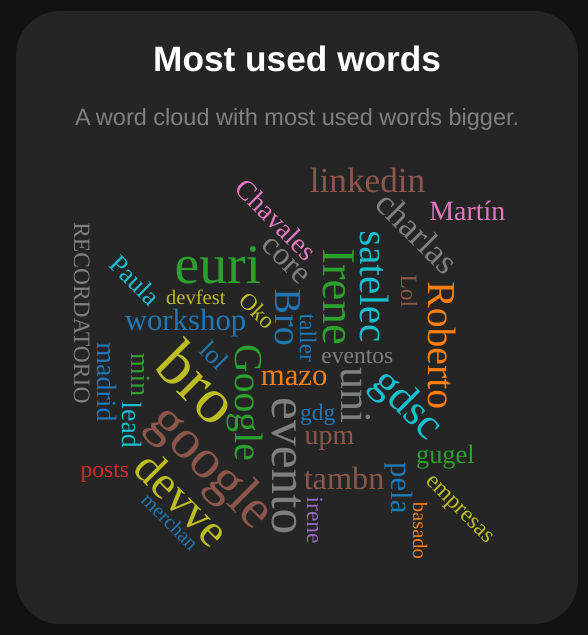
\includegraphics[width=6cm]{img/word_cloud.png} }}
	\qquad
	\subfloat[\centering Nube de emoticonos]{{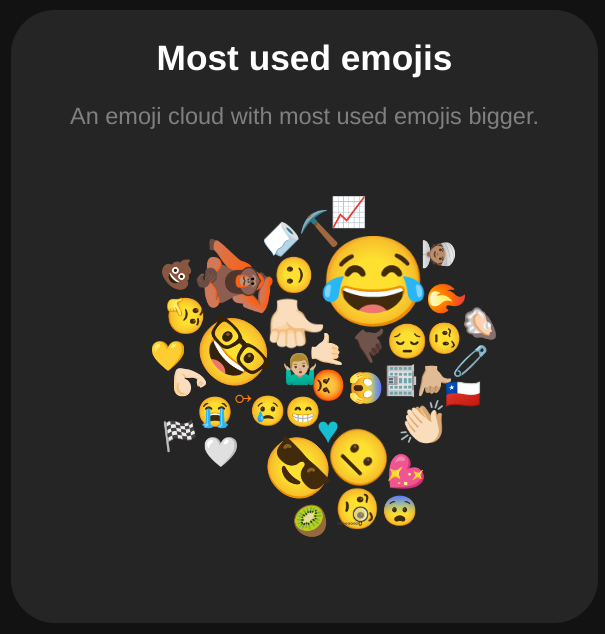
\includegraphics[width=6cm]{img/emoji_cloud.png} }}
	\caption{Ejemplos de los componentes de visualización}
	\label{fig:chap4:visualization_examples}
\end{figure}

Para los gráficos circulares y de barras, se elige la librería \textit{ChartJS}, puesto que cuenta con alta actividad de contribuciones al proyecto, es libre y cuenta con 12 mil estrellas en GitHub. Además, permite alta extensibilidad mediante plugins, de los que hacemos uso, por ejemplo, para mostrar las etiquetas de los datos. Los componentes que uan esta librería adaptan el tamaño del gráfico al número de contactos que hay en el grupo de forma \textit{responsive}. También permiten la interacción con el mismo, pudiendo eliminar contactos de la representación haciendo click sobre el nombre de los mismos en la leyenda.

Por último, como alternativa a los gráficos de berras, se ha planteado también usar un gráfico de araña o radar, pero dicha opción se descarta al observar el solapamiento que tenía lugar con varios contactos.


\subsection{Exportación}

Este módulo permite al usuario exportar tanto la visualización a modo de captura de pantalla, así como la exportación de las métricas calculadas para su uso personal.

\subsubsection{Descargar visualizaciones}

Descargar visualizaciones es un submódulo que permite al usuario descargar como imagen, en formato \textit{png}, las visualizaciones que se muestran en su pantalla.

Como el cliente guarda el estado de las visualizaciones en su \acrshort{dom}, haciendo uso de la librería \textit{html2canvas}, podemos acceder al objeto \textit{body} de la página y obtener una imagen canvas del mismo. Esta imagen no es una captura de pantalla, sino una reconstrucción del objeto \textit{body} del \acrshort{dom}, por lo que puede no ser completamente fiel a la representación que el usuario tiene en su cliente.

Esta imagen se codifica en base64 y se crea un enlace con tipo de contenido (\textit{Content-Type}) \textit{image/png}  para su descarga local desde el navegador.

No se puede hacer uso de la funcionalidad de imprimir pantalla del navegador, puesto que los gráficos usan la etiqueta \acrshort{html} \textit{canvas}, lo que descuadra los gráficos y hace perder formato y colores.

\subsubsection{Descargar resultados}

Del mismo modo que el submódulo anterior, este módulo permite al usuario descargar una versión exportada de los datos y métricas calculadas en formato \acrshort{json} para su posterior uso personal.

Para ello, el submódulo recoge todo el contenido alojado en el estado local del cliente y crea un enlace local para la descarga de los datos. Dicho enlace está compuesto por el tipo de contenido (\textit{Content-Type}) \textit{text/json} seguido del contenido del estado local (en \acrshort{json}) volcado a una cadena de caracteres y codificado para \acrshort{uri}s.

Pueden verse las métricas que se descargan en la \autoref{chap:architecture_metrics}.



\subsection{Tests unitarios}

Los tests unitarios son una parte esencial del proceso de desarrollo de software, ya que ayudan a garantizar que el sistema funciona correctamente y que se cumplen los requisitos funcionales. En nuestro proyecto, hemos desarrollado tests unitarios para asegurarnos de que cada los módulos y submódulos de la aplicación cumplen con lo que se espera de ellos..

Además, los tests unitarios nos ayudan a detectar errores temprano en el proceso de desarrollo, lo que nos permite corregirlos antes de que el sistema sea puesto en producción. También nos permiten validar que la funcionalidad no se ven afectadas cuando se realizan cambios en el código.

En este proyecto, se ha alcanzado una cobertura del 74\% en los tests unitarios, lo que significa que el 74\% del código ha sido cubierto por pruebas. Aunque no se alcanza el 100\% de cobertura, se han desarrollado para los módulos más importantes, como ``Ingesta de datos'', ``Agregadores'' y cálculo de la mayoría de métricas. No se han realizado tests para los componentes de visualización ni el módulo ``Exportador'', puesto que suponen una interacción con el \textit{front-end} y se dejan para futuras líneas de trabajo.

Para el desarrollo de los mismos, se utiliza la librería \textit{Jest}, que permite alta integración con la estructura del proyecto de React, así como asienta las bases para futuras pruebas de componentes visuales que interactúen con los mismos, así como con las rutas de la aplicación.

Para generar los distintos datos de entrada se proveen pequeños archivos de chat maquetados para tipo de fichero. Al mismo tiempo, para los datos de entrada a los distintos componentes lógicos que se prueban, se ha utilizado la librería \textit{faker}, que permite la generación de datos maquetados como nombres, fechas, frases, párrafos y otros; lo cual nos da la posibilidad de generar mensajes al vuelo con la estructura de datos deseada.

A continuación se muestra la ejecución de los tests unitarios:

\begin{figure}[H]
	\centering
	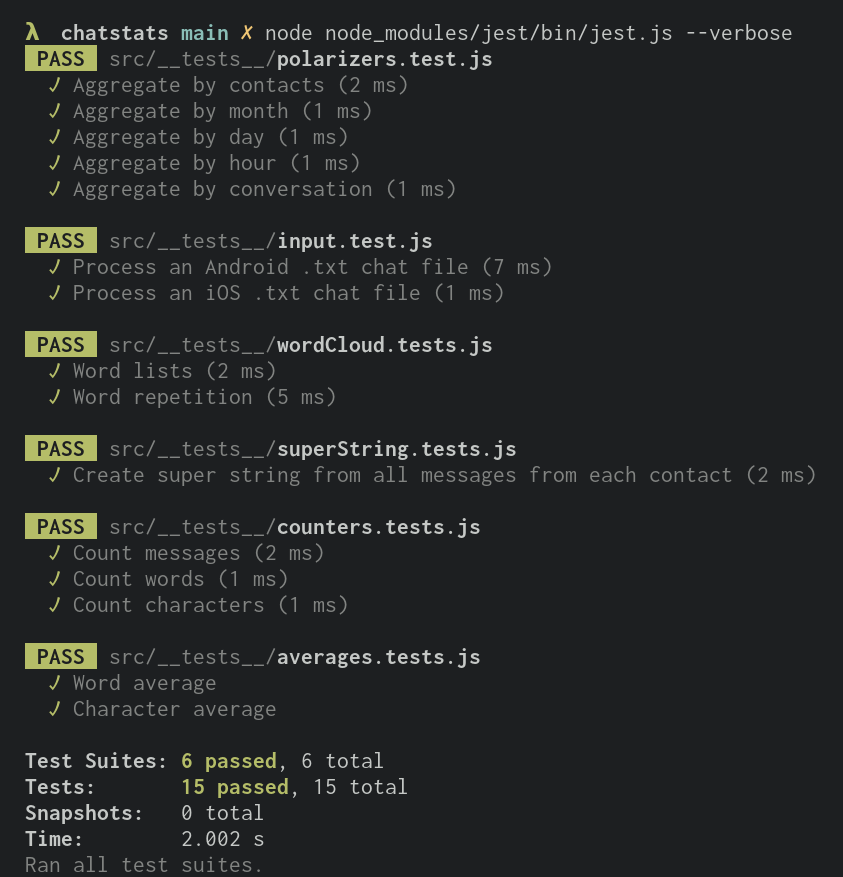
\includegraphics[width=0.6\textwidth]{img/tests.png}
	\caption{Ejecución de tests unitarios}
	\label{fig:chap4:architecture_tests}
\end{figure}